\section{Full Algorithm}\label{Se:fullalg}

Having highlighted the main \Tool\ features, we now describe the complete algorithm.

\subsection{Setup}

The testing session begins by deploying the target app in debug mode. This enables the insertion of debug breakpoints into library APIs. The motivation for this design choice was that it applies to any Android build and any device  (provided the {\tt ro.debuggable} property is set to 1) as opposed to requiring a custom build (as in \cite{EGCCJMS:OSDI10}), which limits applicability and requires heavy maintenance.

Once the target app is deployed, \Tool\ obtains --- via the {\tt apktool} utility --- its manifest file. Parsing the manifest reveals the set of {\tt Activity}s defined by the app that are both public and exported. These are reachable directly via {\tt Intent}s, and so the first IAC inputs created by \Tool\ are benign {\tt Intent}s.

\subsection{Testing Loop}

During testing, \Tool\ switches between 3 modes:
\begin{compactitem}
	\item Monitoring: While a message is being processed by the target input point, \Tool\ tracks via system-level hooks which security-relevant APIs are invoked, and which custom fields the app attempts to access. Monitoring serves both for coverage and for validation purposes.
	\item Testing: When a new field is detected, a probe request is sent for it. Comptabile attack types are then launched. 
	\item Exploration: For a given probe message with boolean extras, variants thereof (with one extra flag toggled at a time) are also sent as probes.
\end{compactitem}
Interleaving monitoring, testing and exploration yields an iterative testing cycle. As custom fields and fresh execution paths are incrementally discovered, the attack surface expands. On the other hand, submitting probe and test messages reveals more custom fields and execution paths. 

To validate the success of a security test, \Tool\ relies on externally observable indications, such as component/application crashes, as well as on the following: 
\begin{compactenum}
	\item Code monitoring: Detection monitors are used also for validation.
	Values reaching security-sensitive operations are observed via run-time handlers 
	triggered in response to hitting debug breakpoints.
	\item Log listener: \Tool\ tracks updates to the standard log files provided by the Android platform. 
	\item HTTP listener: A second output that \Tool\ listens on is outbound HTTP traffic. This method is used primarily to validate XAS vulnerabilities.
\end{compactenum} 
Thanks to these varied validation methods, \Tool\ is able to generate actionable security warnings. These include both (i) detailed code-level artifacts (call stack) and (ii) a concrete attack vector (both payload and entrypoint). An example of such a report appears in \figref{screenshot}.

\begin{figure}
	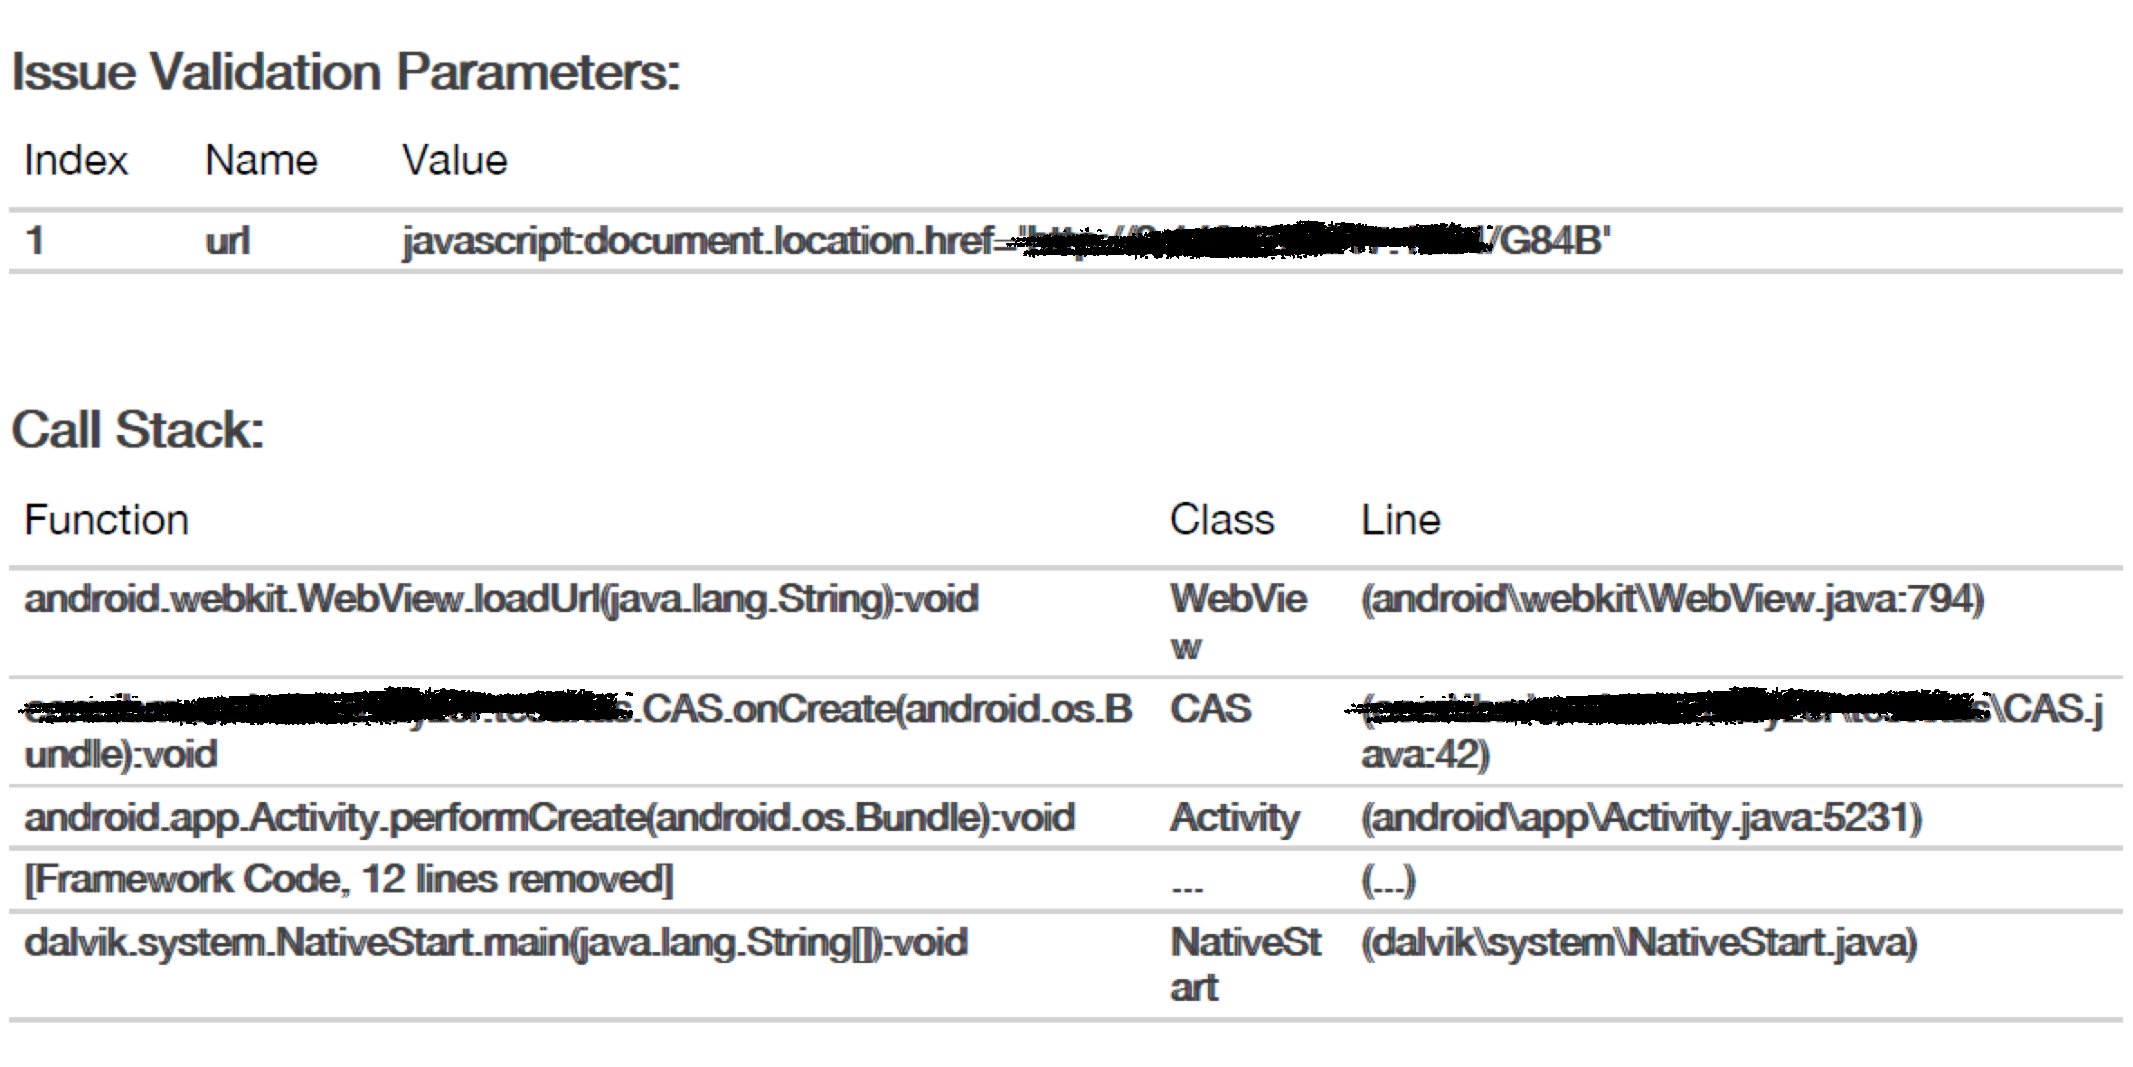
\includegraphics[width=\columnwidth]{screenshot.pdf}
	\caption{\label{Fi:screenshot}A Vulnerability Report Output by \Tool}
\end{figure} 

\subsection{Formal Description}

\algref{maalg} summarizes the complete flow of the \Tool\ algorithm. The starting point is to instrument the target app to record (select) library calls as well as accesses to user-provided data. Next, \Tool\ obtains the declared IAC input points $E$ of the subject application via analysis of its manifest. These seed the iterative testing process. The fixpoint loop iterates over $E$, picking at each iteration a candidate input point $e$ and removing it from the worklist.

\begin{algorithm}[t]
	\DontPrintSemicolon
	\SetKwInOut{Input}{Input}
	\SetKwInOut{Output}{Output}
	\KwIn{$(D,M,V,I)$ \tcp*[h]{testing capabilities}}\;
	\KwIn{$A$ \tcp*[h]{subject mobile app}}\;
	\KwOut{$O$ \tcp*[h]{detected vulnerabilities}}\;
	\Begin{
		$A' \longleftarrow I(A)$ \tcp*[h]{instrument $A$}\; \\
		$E$ $\longleftarrow$ declared interface points of $A$\; \\
		$O \longleftarrow \emptyset$\; \\
		\While{$E \neq \emptyset$}{
			$e$ $\longleftarrow$ choose from $E$\; \\
			$E \longleftarrow E \setminus \{ e \}$\; \\
			\ForEach{$m \in M(e)$}{
				{$b \longleftarrow D(m,e)$}\; \\
				\If{$b$}{
					$p[m,e] \longleftarrow \text{create payload for $e$ with $m$}$\; \\
					$(r,E') \longleftarrow \text{fire $p[m,e]$}$\; \\
					$E \longleftarrow E \cup E'$\; \\
					\If{$V(r)$}{
						$O \longleftarrow O \cup \{ r \}$\;
					}
				}
			}
		}
	}
	\caption{\label{Al:maalg}{\bf Outline of the Core \Tool\ Algorithm, where $D$, $M$, $V$ and $I$ Denote Detection, Mutation, Validation and Instrumentation, Respectively}}
\end{algorithm}


For the current input point $e$, the next step is to check whether $e$ satisfies the necessary conditions for each attack type $m$. This is represented as the $D(m,e)$ call. Successful detection leads to the creation and application of a payload $p[m,e]$. Exercising the instrumented app $A'$ with $p[m,e]$ yields two artifacts: additional input points $E'$ (discovered by monitoring accesses to custom parameters) and recording of app behaviors/outputs $r$ for validation. The set $O$ of vulnerabilities reported by \Tool\ is augmented if $r$ confirms a vulnerability (the $V(r)$ check).

While \Tool\ is a dynamic testing system with (purposely) limited means to track the internal behavior of the target app, there are still situations in which full coverage is guaranteed. These are governed by a simplifying assumption, stated formally in Definition \ref{De:dataind}, which is too idealized to hold pervasively in reality, but still (i) provides insight into the design of \Tool, and (ii) appears useful in practice given \Tool's recall rate of $>90\%$ over a large set of popular Android apps. (See \secref{evaluation}.)

\begin{definition}[Data Independence]\label{De:dataind} We refer to input point $e$ in the IAC interface as \emph{data independent} if execution flow starting at $e$ is decided solely according to (i) boolean extras and/or (ii) presence of extra fields. In particular, the values of non-boolean extras (and other variables in the program) do not affect control flow (cf. \cite{SYGABSV:ISSTA14,W:POPL86}).
\end{definition}

\begin{theorem}[Coverage] Let input point $e$ be data independent, s.t. the value of incoming IAC field $f$, arriving through $e$, flows into sink $s$. 
	Denote by \ETool\ the naive version of \Tool, which enumerates all possible combinations of boolean extras.
	Then \ETool\ is guaranteed to reach $s$ with $f$ mapped to a test payload.\footnote{
		This claim is trivially extensible to \Tool\ by further assuming that boolean extras are related either via independence or via domination.
	}
	\begin{proof}[Sketch] \ETool\ systematically enumerates all boolean combinations. This --- conjoined with the assumption that $e$ is data independent --- guarantees that at some point access to $f$ will be observed. Thus, $f$ will become an attack target (where only the presence, but not the value, of $f$ affects control flow). All continuations of the execution prefix leading to $f$ will be enumerated, which guarantees that a path $p$ starting at $e$, going through a read of $f$ and ending at $s$ will be traversed. Given $f$ is a non-boolean field, \ETool\ will initiate a test execution of $p$ with $f$ mapped to a test payload, which completes the proof.
	\end{proof}
\end{theorem}